\begin{figure}
  \centering
  \begin{tikzpicture}
    \node at (0, 0){
      \includegraphics[width=6cm]{experiments/kitti/vae_occ_aml/15_long/results_1}
    };
    \node at (0, -2.5){
      \includegraphics[width=6cm]{experiments/kitti/vae_occ_aml/15_long_statistics/results_1}
    };
    \node at (0, -5){
      \includegraphics[width=6cm]{experiments/kitti/vae_occ_aml/15_long_statistics_combined/results_1}
    };
   
    \node at (6.25, 0){
      \includegraphics[width=6cm]{experiments/kitti/vae_occ_aml/15_long/results_4}
    };
    \node at (6.25, -2.5){
      \includegraphics[width=6cm]{experiments/kitti/vae_occ_aml/15_long_statistics/results_4}
    };
    \node at (6.25, -5){
      \includegraphics[width=6cm]{experiments/kitti/vae_occ_aml/15_long_statistics_combined/results_4}
    };
    
    \draw[-,dashed] (-3.25, -1.25) -- (9.5,-1.25);
    \draw[-,dashed] (-3.25, -3.75) -- (9.5,-3.75);
    
    %\node at (10,0) {
    %  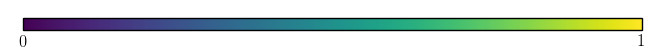
\includegraphics[height=2.5cm]{experiments/3d/vae_occ/easy_15/colorbar}
    %};
    
    \node at (3.25, 1.5) {reconstruction};
    \node[rotate=90] at (-3.5, 0) {\AML};
    \node[rotate=90] at (-3.75, -2.5) {\begin{tabular}{c}\AML\\+weights\end{tabular}};
    \node[rotate=90] at (-4, -5) {\begin{tabular}{c}\AML\\+weights\\+combined\end{tabular}};
  \end{tikzpicture}

  % TODO short caption
  \caption{Qualitative results for \AML on the extracted KITTI dataset. We demonstrate
  the influence of using the weights $\rho_i$ marked as +weights; here, the weights are
  pre-computed on ShapeNet as discussed for Equation \eqref{eq:experiments-3d-weights}.
  Additionally we show the influence of training the prior on both ShapeNet training sets,
  referred to as +combined. As always, we show horizontal slices for the observed points,
  the corresponding partial free space and the predictions.
  }
  \label{fig:experiments-kitti-aml-1}
\end{figure}

\begin{figure}
  \centering
  %\hspace*{-1.5cm}
  \begin{tikzpicture}
    \node at (0, 0) {
      \includegraphics[width=3.75cm,trim={3.5cm 2.5cm 3.5cm 2.5cm},clip]{experiments/kitti/vae_occ_aml/15_long_statistics_combined/0_input_45}
    };
    \node at (3.5, 0) {
      \includegraphics[width=3.75cm,trim={3.5cm 2.5cm 3.5cm 2.5cm},clip]{experiments/kitti/vae_occ_aml/15_long_statistics_combined/0_prediction_45}
    };
    \node at (7, 0) {
      \includegraphics[width=3.75cm,trim={3.5cm 2.5cm 3.5cm 2.5cm},clip]{experiments/kitti/baseline/moderate_15/0_prediction_45}
    };

    % \node at (7, 0) {
    %   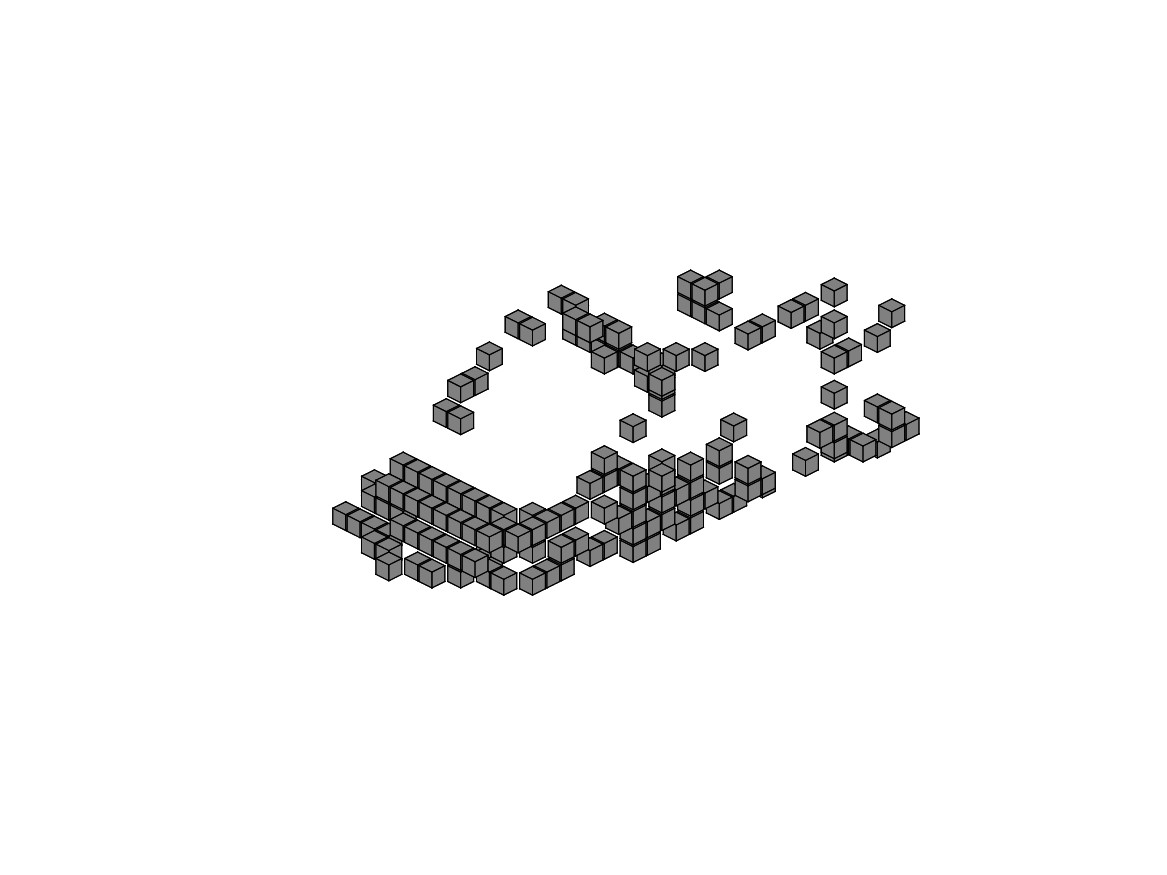
\includegraphics[width=3.75cm,trim={3.5cm 2.5cm 3.5cm 2.5cm},clip]{experiments/kitti/vae_occ_aml/15_long_statistics_combined/2_input_135}
    % };
    % \node at (10.5, 0) {
    %   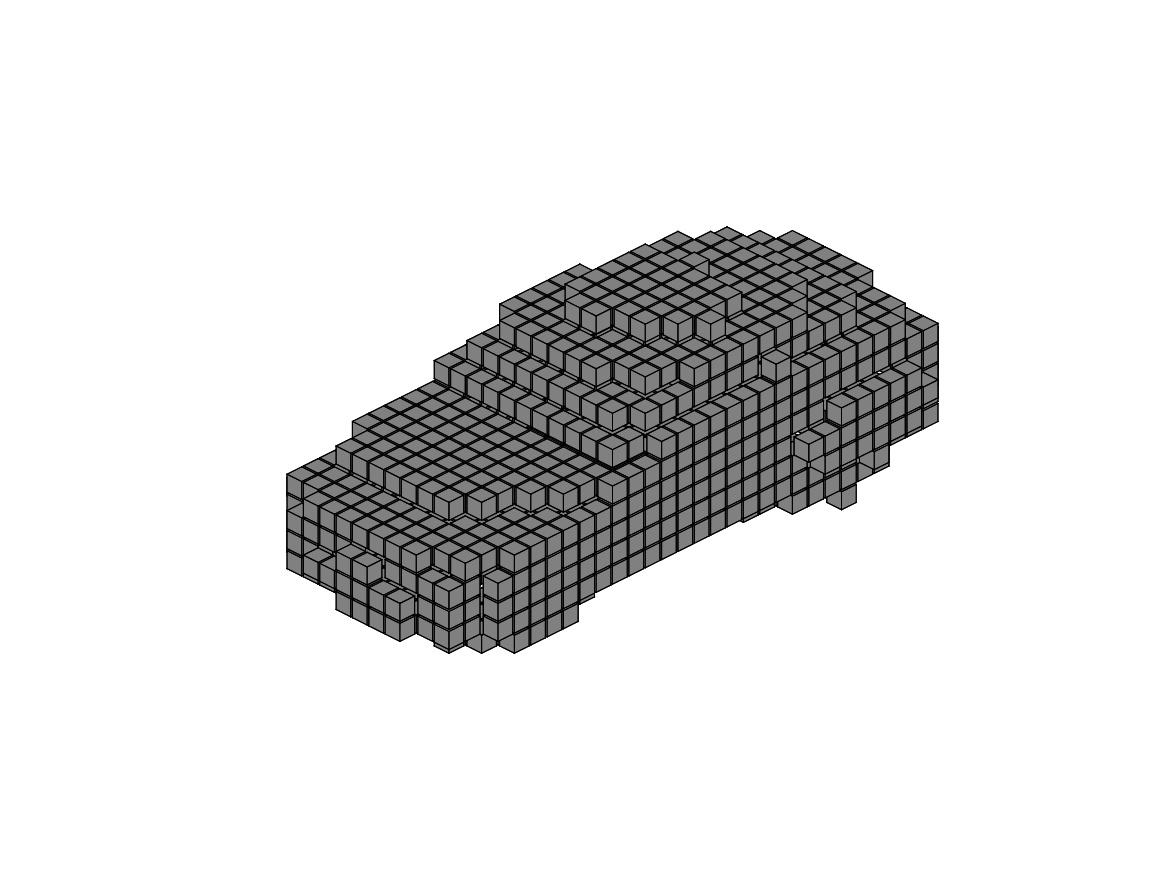
\includegraphics[width=3.75cm,trim={3.5cm 2.5cm 3.5cm 2.5cm},clip]{experiments/kitti/vae_occ_aml/15_long_statistics_combined/2_prediction_135}
    % };
    
    \node at (0, -3) {
      \includegraphics[width=3.75cm,trim={3.5cm 2.5cm 3.5cm 2.5cm},clip]{experiments/kitti/vae_occ_aml/15_long_statistics_combined/1_input_45}
    };
    \node at (3.5, -3) {
      \includegraphics[width=3.75cm,trim={3.5cm 2.5cm 3.5cm 2.5cm},clip]{experiments/kitti/vae_occ_aml/15_long_statistics_combined/1_prediction_45}
    };
    \node at (7, -3) {
      \includegraphics[width=3.75cm,trim={3.5cm 2.5cm 3.5cm 2.5cm},clip]{experiments/kitti/baseline/moderate_15/1_prediction_45}
    };

    % \node at (7, -3) {
    %   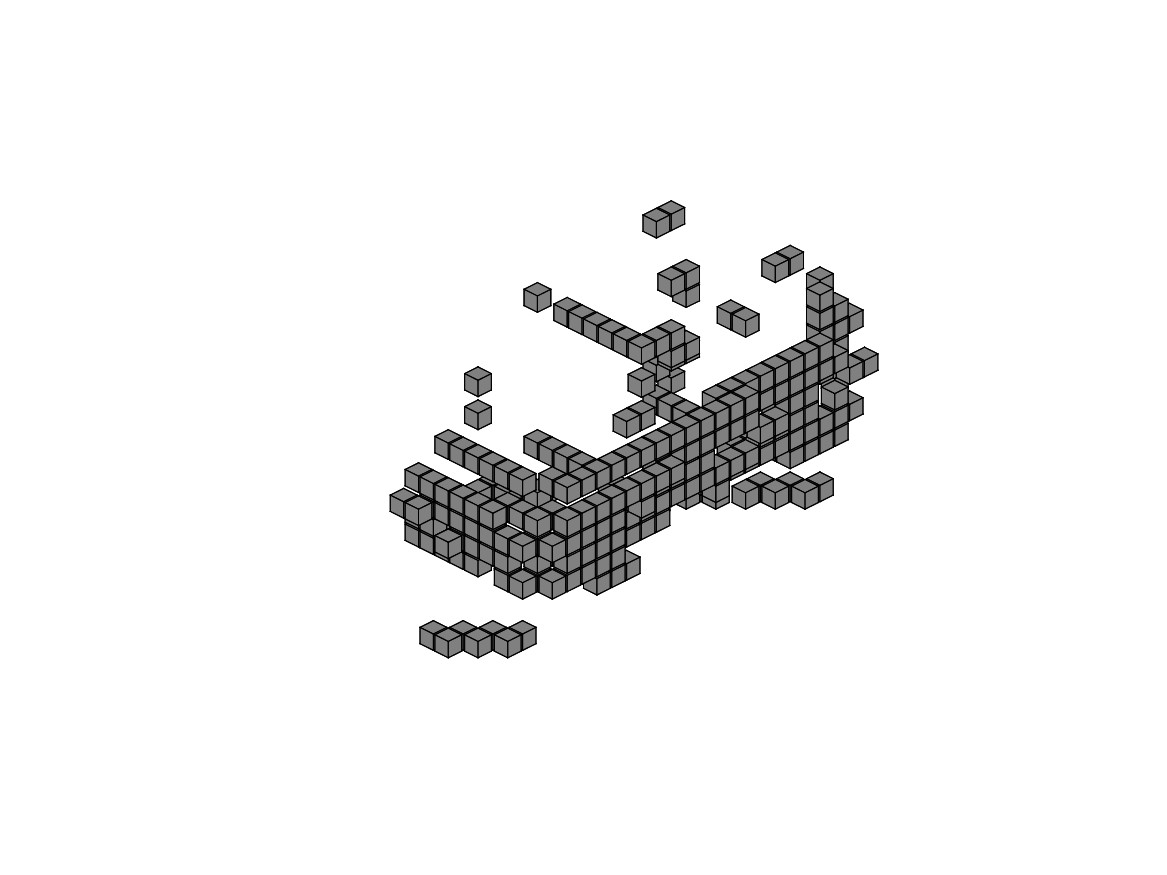
\includegraphics[width=3.75cm,trim={3.5cm 2.5cm 3.5cm 2.5cm},clip]{experiments/kitti/vae_occ_aml/15_long_statistics_combined/0_input_135}
    % };
    % \node at (10.5, -3) {
    %   \includegraphics[width=3.75cm,trim={3.5cm 2.5cm 3.5cm 2.5cm},clip]{experiments/kitti/vae_occ_aml/15_long_statistics_combined/0_prediction_135}
    % };
  
    \node at (0, -6) {
      \includegraphics[width=3.75cm,trim={3.5cm 2.5cm 3.5cm 2.5cm},clip]{experiments/kitti/vae_occ_aml/15_long_statistics_combined/2_input_45}
    };
    \node at (3.5, -6) {
      \includegraphics[width=3.75cm,trim={3.5cm 2.5cm 3.5cm 2.5cm},clip]{experiments/kitti/vae_occ_aml/15_long_statistics_combined/2_prediction_45}
    };
    \node at (7, -6) {
      \includegraphics[width=3.75cm,trim={3.5cm 2.5cm 3.5cm 2.5cm},clip]{experiments/kitti/baseline/moderate_15/2_prediction_45}
    };

    % \node at (7, -6) {
    %   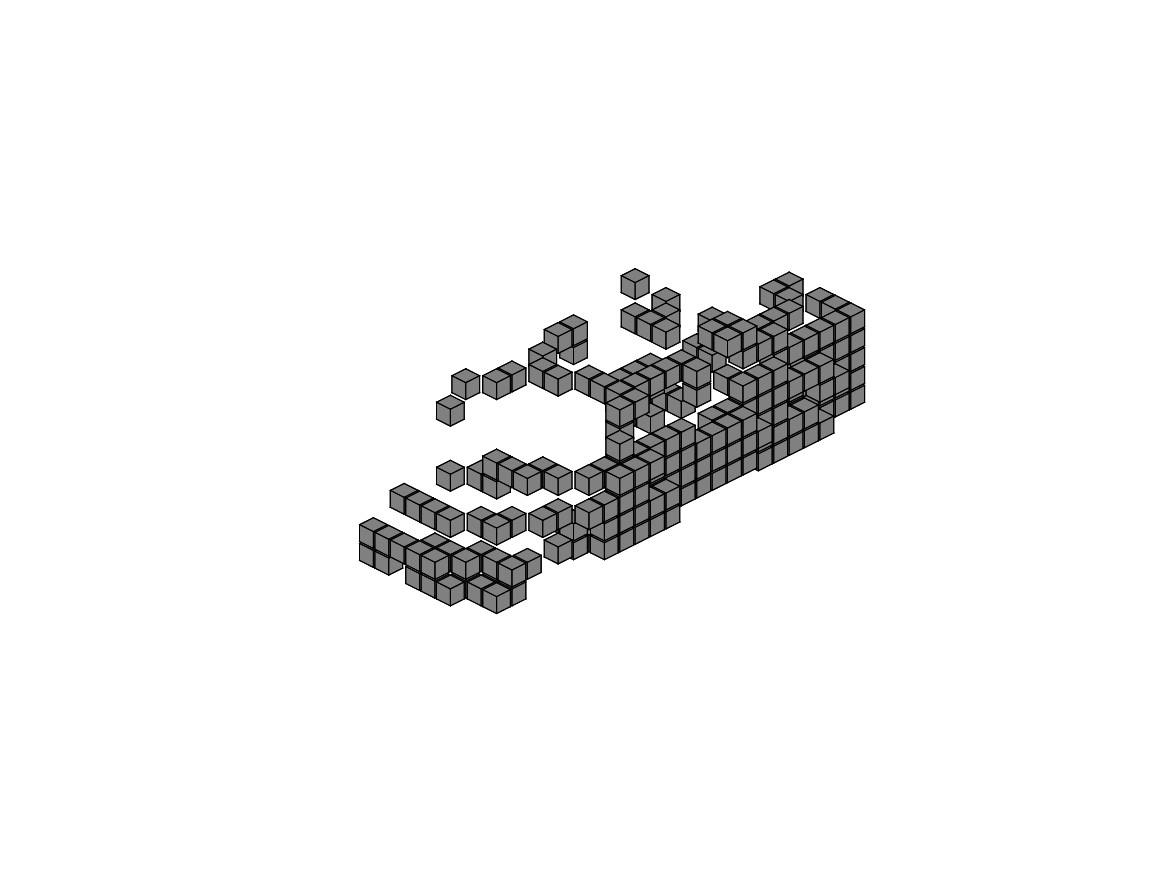
\includegraphics[width=3.75cm,trim={3.5cm 2.5cm 3.5cm 2.5cm},clip]{experiments/kitti/vae_occ_aml/15_long_statistics_combined/1_input_135}
    % };
    % \node at (10.5, -6) {
    %   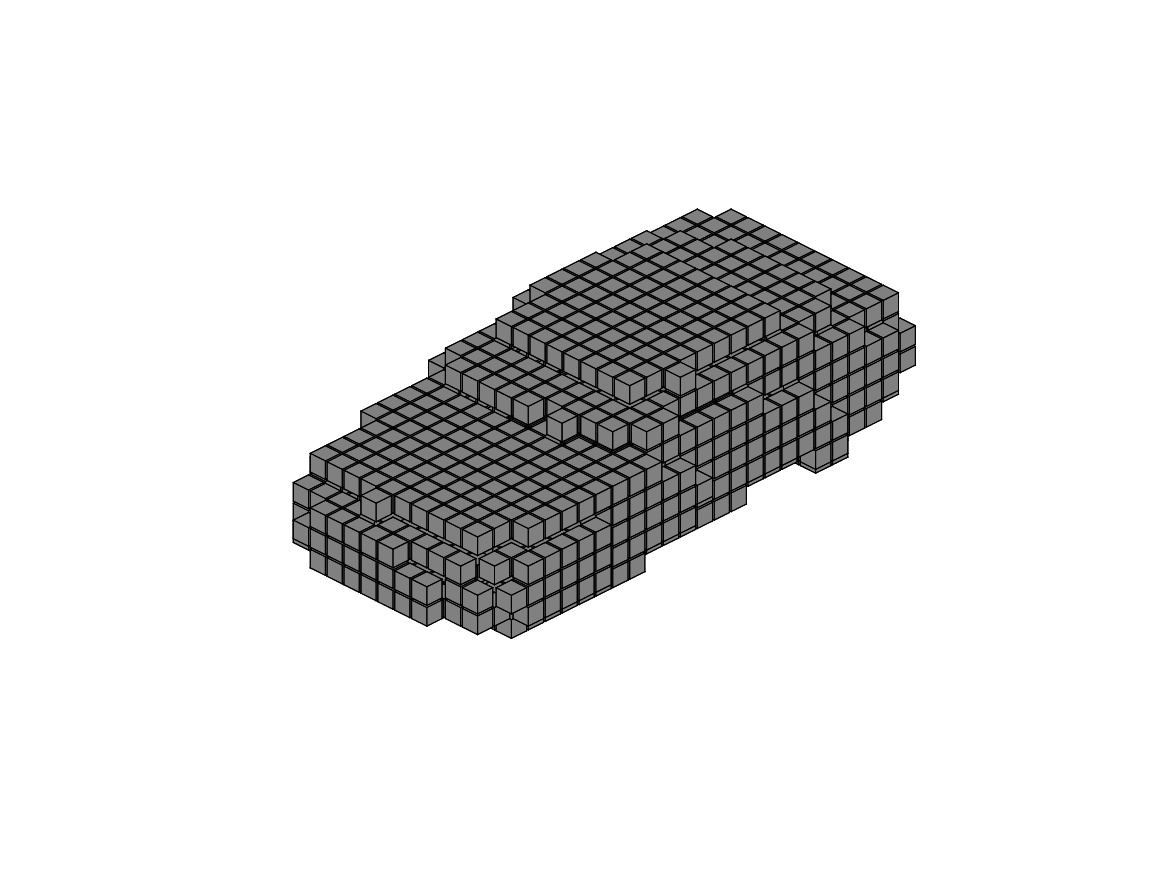
\includegraphics[width=3.75cm,trim={3.5cm 2.5cm 3.5cm 2.5cm},clip]{experiments/kitti/vae_occ_aml/15_long_statistics_combined/1_prediction_135}
    % };
    
    \node at (0, -9) {
      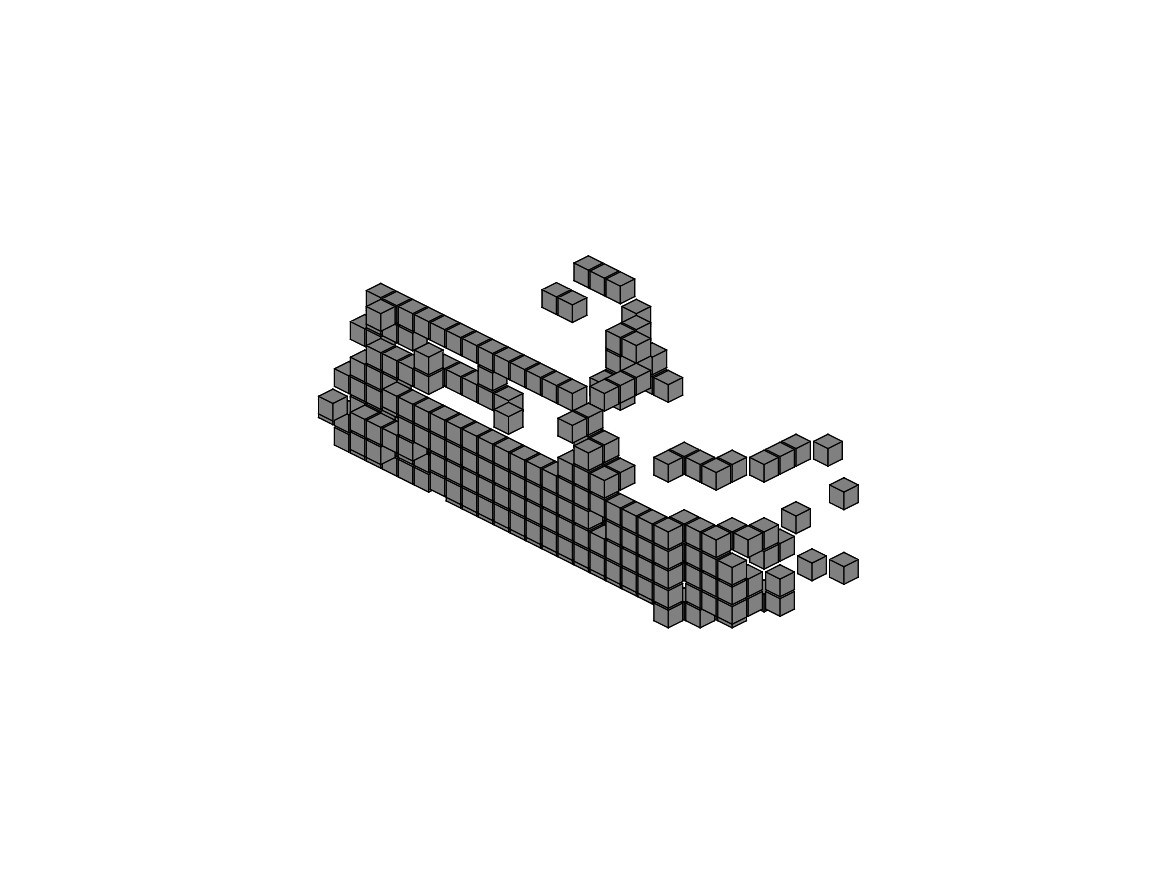
\includegraphics[width=3.75cm,trim={3.5cm 2.5cm 3.5cm 2.5cm},clip]{experiments/kitti/vae_occ_aml/15_long_statistics_combined/3_input_45}
    };
    \node at (3.5, -9) {
      \includegraphics[width=3.75cm,trim={3.5cm 2.5cm 3.5cm 2.5cm},clip]{experiments/kitti/vae_occ_aml/15_long_statistics_combined/3_prediction_45}
    };
    \node at (7, -9) {
      \includegraphics[width=3.75cm,trim={3.5cm 2.5cm 3.5cm 2.5cm},clip]{experiments/kitti/baseline/moderate_15/3_prediction_45}
    };

    % \node at (7, -9) {
    %   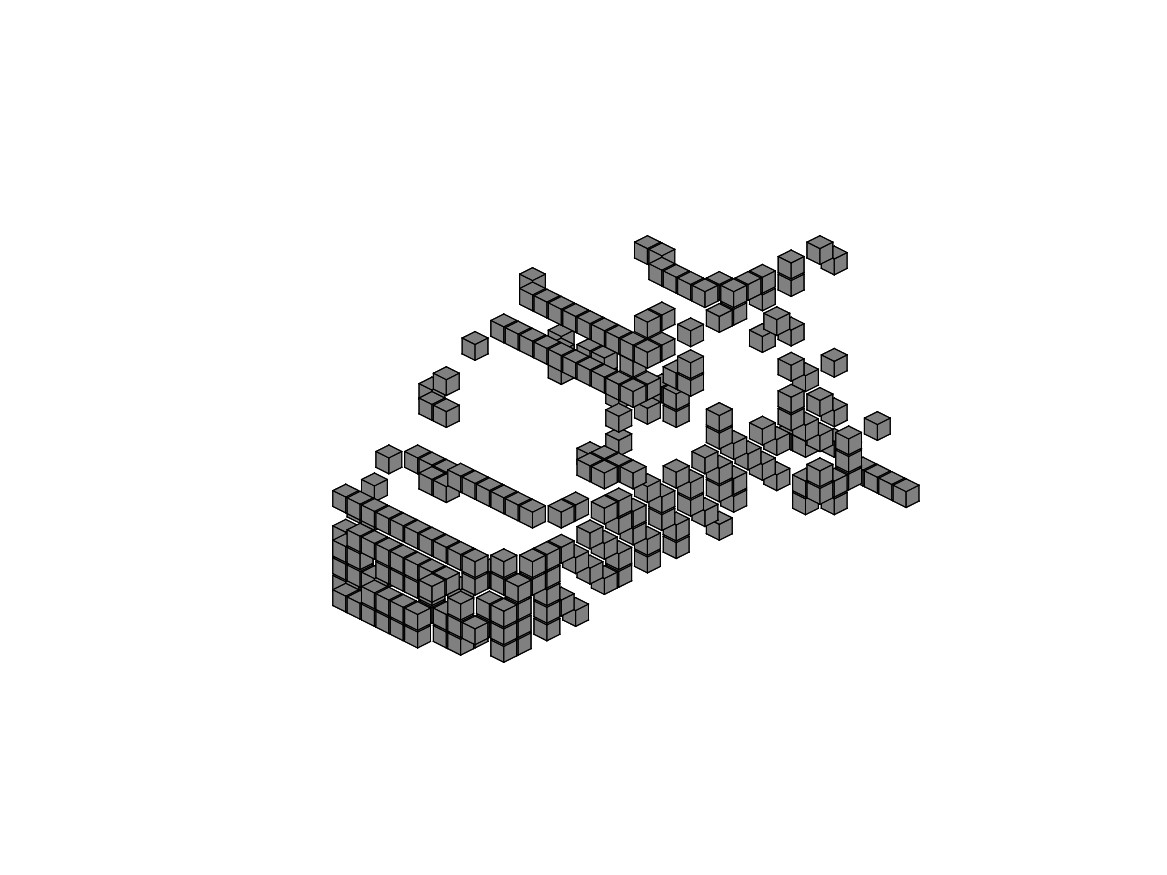
\includegraphics[width=3.75cm,trim={3.5cm 2.5cm 3.5cm 2.5cm},clip]{experiments/kitti/vae_occ_aml/15_long_statistics_combined/4_input_135}
    % };
    % \node at (10.5, -9) {
    %   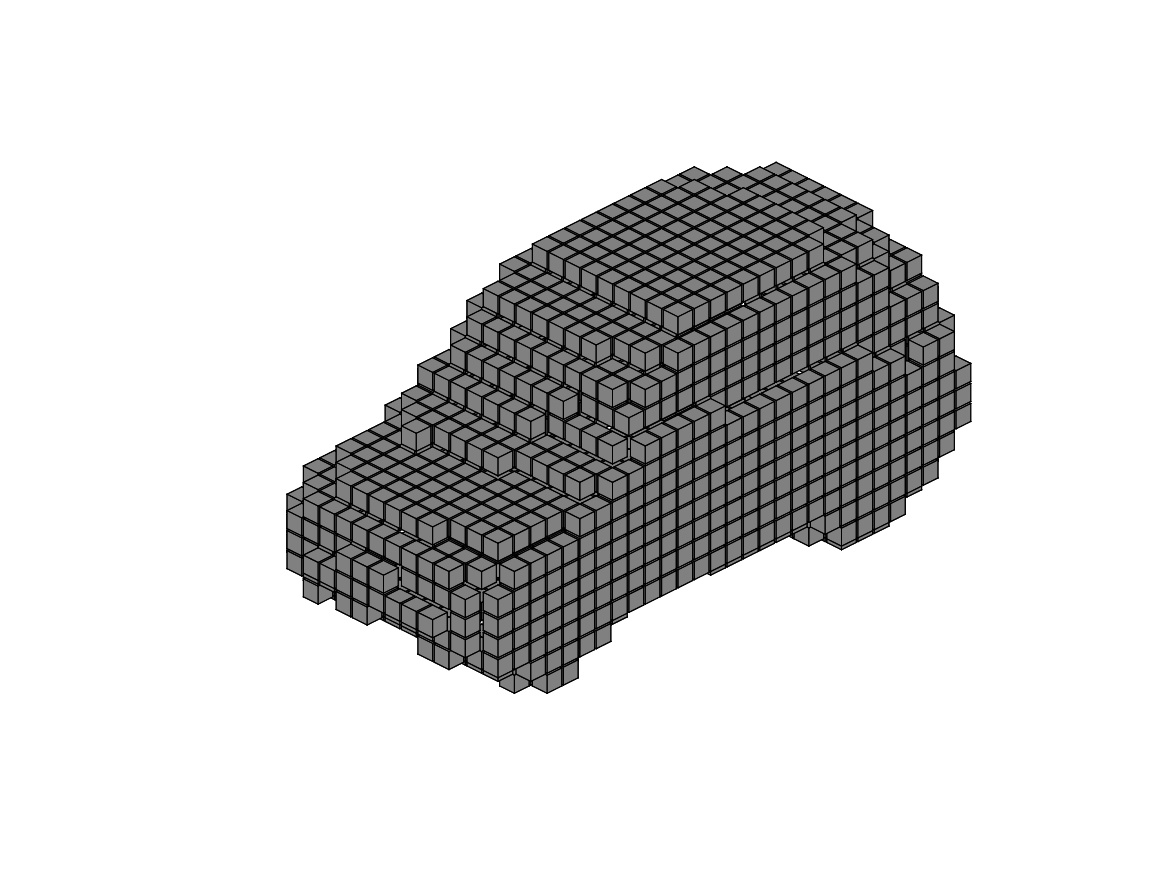
\includegraphics[width=3.75cm,trim={3.5cm 2.5cm 3.5cm 2.5cm},clip]{experiments/kitti/vae_occ_aml/15_long_statistics_combined/4_prediction_135}
    % };
    
    \node at (0, -12) {
      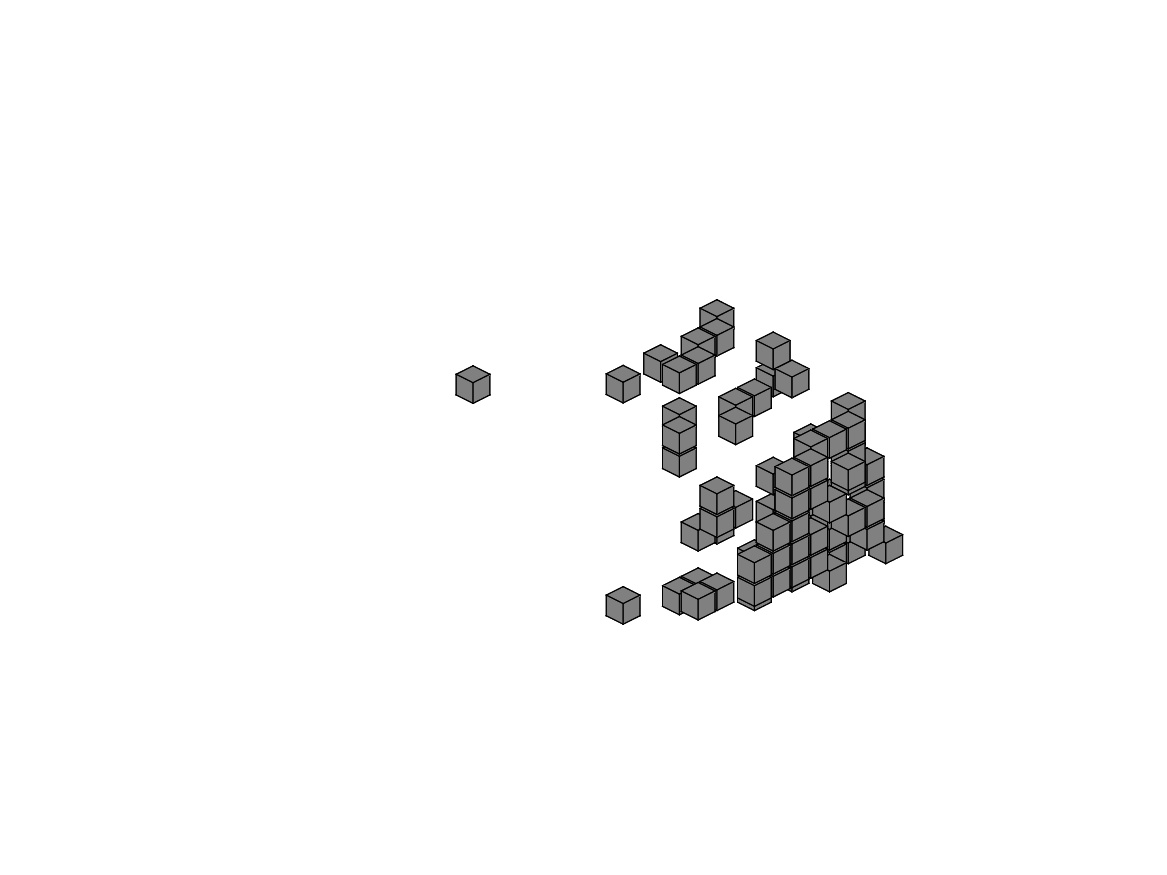
\includegraphics[width=3.75cm,trim={3.5cm 2.5cm 3.5cm 2.5cm},clip]{experiments/kitti/vae_occ_aml/15_long_statistics_combined/4_input_45}
    };
    \node at (3.5, -12) {
      \includegraphics[width=3.75cm,trim={3.5cm 2.5cm 3.5cm 2.5cm},clip]{experiments/kitti/vae_occ_aml/15_long_statistics_combined/4_prediction_45}
    };
    \node at (7, -12) {
      \includegraphics[width=3.75cm,trim={3.5cm 2.5cm 3.5cm 2.5cm},clip]{experiments/kitti/baseline/moderate_15/4_prediction_45}
    };

    \node at (0, 1.75) {Input};
    \node at (3.5, 1.75) {\AML};
    \node at (7, 1.75) {Baseline};
  \end{tikzpicture}

  % TODO short caption
  \caption{Comparison of \AML and the supervised baseline on KITTI; here,
  \AML uses occupancy only and we show the observed points and the predicted shapes
  in voxelized form. For both, we show 2 distinct viewpoints. For \AML we show
  two examples. For the latter, we also show the predicted shape using the supervised
  baseline to illustrate that \AML still misses details, \eg along the root.}
  \label{fig:experiments-kitti-aml-2}
\end{figure}
\begin{figure}
  \centering
  \begin{tikzpicture}
    \node at (0, 0) {
      \includegraphics[width=3.75cm,trim={3.5cm 2.5cm 3.5cm 2.5cm},clip]{experiments/kitti/vae_occ_sdf_aml/15_statistics_combined_075/0_input_45}
    };
    \node at (3.5, 0) {
      \includegraphics[width=3.75cm,trim={3.5cm 2.5cm 3.5cm 2.5cm},clip]{experiments/kitti/vae_occ_sdf_aml/15_statistics_combined_075/0_prediction_45}
    };
    \node at (8, 0) {
      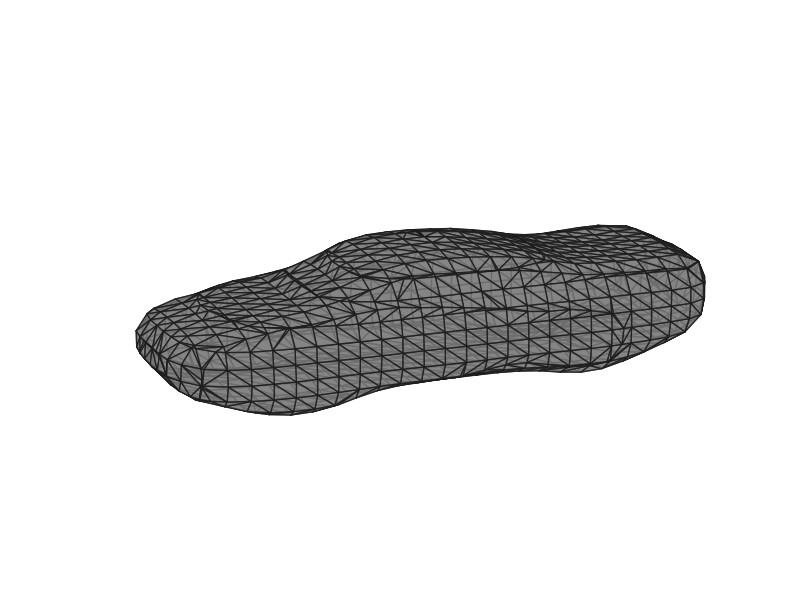
\includegraphics[width=3.75cm,trim={1cm 3cm 1cm 3cm},clip]{experiments/kitti/vae_occ_sdf_aml/15_statistics_combined_075/0_prediction}
    };
    
    \node at (0, -3) {
      \includegraphics[width=3.75cm,trim={3.5cm 2.5cm 3.5cm 2.5cm},clip]{experiments/kitti/vae_occ_sdf_aml/15_statistics_combined_075/1_input_45}
    };
    \node at (3.5, -3) {
      \includegraphics[width=3.75cm,trim={3.5cm 2.5cm 3.5cm 2.5cm},clip]{experiments/kitti/vae_occ_sdf_aml/15_statistics_combined_075/1_prediction_45}
    };
    \node at (8, -3) {
      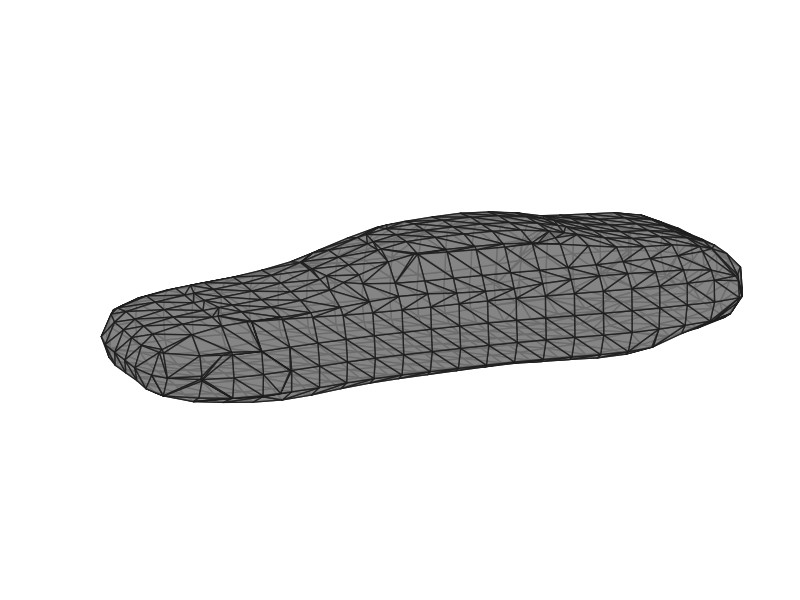
\includegraphics[width=3.75cm,trim={1cm 3cm 1cm 3cm},clip]{experiments/kitti/vae_occ_sdf_aml/15_statistics_combined_075/1_prediction}
    };

    \node at (0, -3) {
      \includegraphics[width=3.75cm,trim={3.5cm 2.5cm 3.5cm 2.5cm},clip]{experiments/kitti/vae_occ_sdf_aml/15_statistics_combined_075/2_input_45}
    };
    \node at (3.5, -3) {
      \includegraphics[width=3.75cm,trim={3.5cm 2.5cm 3.5cm 2.5cm},clip]{experiments/kitti/vae_occ_sdf_aml/15_statistics_combined_075/2_prediction_45}
    };
    \node at (8, -3) {
      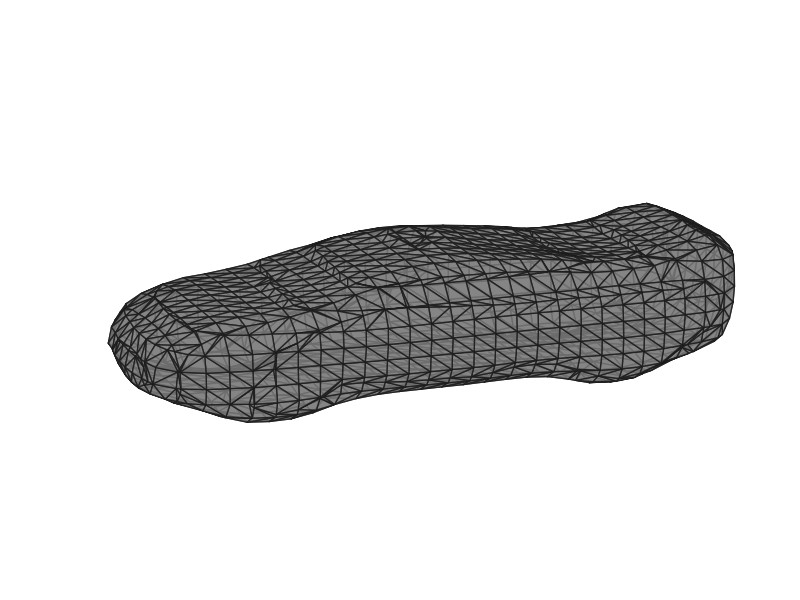
\includegraphics[width=3.75cm,trim={1cm 3cm 1cm 3cm},clip]{experiments/kitti/vae_occ_sdf_aml/15_statistics_combined_075/2_prediction}
    };
    
    \node at (0, 1.85) {input};
    \node at (3.5, 1.85) {prediction};
    \node at (8, 1.85) {mesh};
  \end{tikzpicture}

  % TODO short caption
  \caption{3D vsualizations of the predicted shapes using \AML predicting
  both occupancy and signed distance functions. The meshes on the right
  were derived using marching cubes.}
  \label{fig:experiments-kitti-aml-3}
\end{figure}
